% Copyright (c) 2014,2016 Casper Ti. Vector
% Public domain.

\chapter{序言}

\section{研究问题与目标}
本研究的研究目标是解决深度学习应用在嵌入式平台上开发的难度与低效的问题。嵌入式平台相对于传统的GPU或者CPU集群而言,系统偏底层,开发难度大,有些嵌入式平台需要具有硬件编程背景的开发人员才能充分优化其性能。此外,嵌入式平台的处理器效率,内存上限,使用环境都有许多限制,传统的深度学习应用必须经过充分的修改和调优才能运行于嵌入式平台上。

本研究的目标是设计并实现一种深度学习框架,在开发的效率与计算性能两个方面优化嵌入式平台上的深度学习应用。该框架应该具有通用性,兼容性,以及便捷性等等特点,让深度学习的研究人员在不需要嵌入式设备的相关背景即可立刻上手,基于其他平台的深度学习应用也可以方便地迁移到嵌入式设备。该框架的实现应同时具有高的计算性能,能在运算过程中主动使用嵌入式平台上的硬件加速单元和接口。

\section{选题背景与意义}

\begin{figure}[!ht]
	\centering
	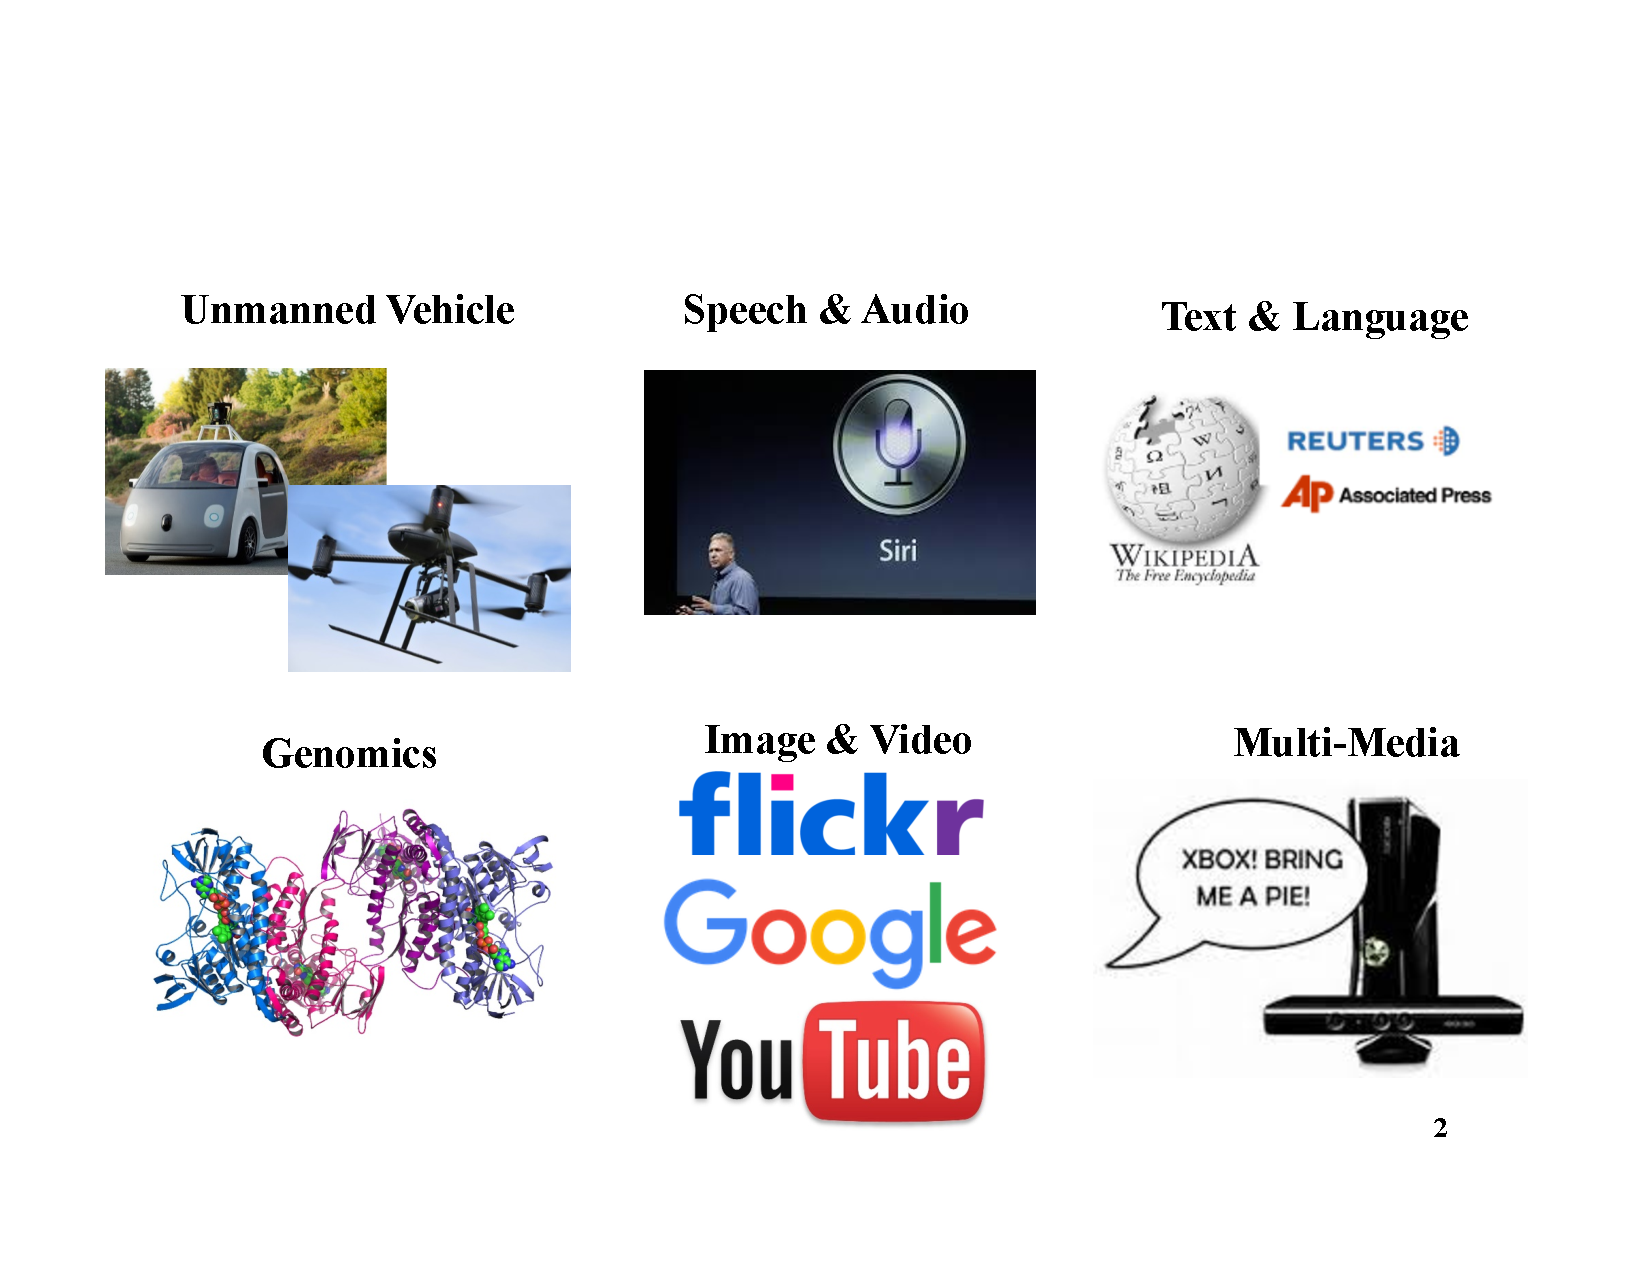
\includegraphics[width=0.8\textwidth]{assets/imgs/deeplearning.pdf}
	\label{fig:deeplearning}
	\caption{深度学习的应用领域\protect\footnotemark}
\end{figure}

\footnotetext{\url{http://cadlab.cs.ucla.edu/~cong/slides/HALO15_keynote.pdf}}

近年来,深度学习应用在各种领域中,比如图像识别、语音识别、文本和语言分析等等,并取得了突出的成果:在ImageNet大规模视觉识别挑战(Large Scale Visual Recognition Challenge,简称LSVRC)2012年的比赛中,多伦多大学的Alex Krizhevsky\supercite{krizhevsky2012imagenet}等人使用了大规模的卷积神经网络对ImageNet进行训练并取得了惊人的成绩。2016年3月,Google DeepMind公司设计的AlphaGo围棋机器人\supercite{silver2016mastering}利用深度学习与蒙特卡洛搜索的方法,以4-1的成绩打败了棋手李世乭。此外,深度学习也逐渐应用于医疗、教育、商业等其他大规模的数据分析等等领域,为改善人们的生活做出了突出的贡献。

上述深度学习的应用领域主要基于大规模的硬件系统,使用GPU或者集群等等技术进行机器学习算法训练与计算的加速。最近随着自动驾驶汽车和无人机等小型无人设备的兴起,这类设备也开始使用深度学习优化已有的SLAM和计算机视觉等算法。这类设备由于面积和重量的限制,只能使用小型的、乃至于微型的嵌入式设备进行计算。嵌入式设备的性能远低于传统深度学习应用所利用的GPU等平台,因此对这类小型设备需要使用的深度学习算法进行优化是必要的。

\section{论文结构安排}

本论文的结构安排如下:

第一章:序言,简单介绍本研究的问题背景与研究目标,以及研究的意义和价值。

第二章:背景知识,介绍深度学习和神经网络、SoC、FPGA和高层次综合的基本原理。

第三章:使用技术,介绍本研究所使用到的几种技术,包含:Zynq SoC平台,SDSoC开发工具和深度学习框架Caffe等等。

第四章:本章是论文的核心和重点,主要介绍SoCaffe的实现。首先给出SoCaffe的系统设计,主要包含对Caffe的计算特性的分析,以及软硬件划分的方式;之后,重点介绍FPGA加速GEMM计算的方式,以及各种优化策略的原理和设计;最后给出Caffe软件端的编译和整个系统的生成。

第五章:实验结果与分析,分别测试GEMM加速器和SoCaffe的整体性能测试与分析,使用常用的MNIST深度学习应用进行SoCaffe的可用性测试。

结论:根据实验结果的分析做出总结,并给出下一步工作的展望。

% vim:ts=4:sw=4
